% =====================================================================
% DEXTRA - IEEE conference paper
%
% Compile:  Overleaf (upload this folder, set compiler to pdfLaTeX)
%           or locally:  pdflatex main && pdflatex main
%
% Every number in Sections III and V is taken from the generated tables
% in tables/, which notebooks 08-10 produced. Do not retype them by hand;
% if a number changes, regenerate the table and it changes here too.
%
% WHAT STILL NEEDS YOU:
%   - Section II (Related Work) is a scaffold. The references below are a
%     starting set; you must verify each one and add the air-quality
%     forecasting literature.
%   - Author block.
%   - Anything marked \todo{}.
% =====================================================================
\documentclass[conference]{IEEEtran}

\usepackage{graphicx}
\usepackage{booktabs}
\usepackage{amsmath}
\usepackage{amssymb}
\usepackage{url}
\usepackage{cite}

\graphicspath{{figures/}}

% TODOs are deliberately loud so none survives to submission.
\newcommand{\todo}[1]{\textbf{[TODO: #1]}}

\begin{document}

\title{Forecasting Severe Air-Quality Days in Cities with No Monitoring
History: A Leave-One-City-Out Study Across India}

\author{\IEEEauthorblockN{\todo{author name}}
\IEEEauthorblockA{\todo{department, institution}\\
\todo{city, country}\\
\todo{email}}}

\maketitle

\begin{abstract}
Air-quality forecasts are most valuable in cities with no monitoring history, yet
such cities are precisely the ones excluded when a model is trained and tested on the
same place. We evaluate one- to three-day national Air Quality Index (AQI) forecasting
for fifteen Indian cities over seven years (2019--2025, 38{,}355 city-days) under a
strict leave-one-city-out protocol: in each of fifteen folds the held-out city
contributes nothing to training, validation, gap-filling medians or alarm calibration,
and training ends before the evaluation period begins. We compare a persistence
reference, a training-free nightly anchor, gradient boosting, an LSTM, DLinear,
PatchTST, an inverted transformer and two zero-shot time-series foundation models
against a model that anchors its forecast on the last observed AQI and additionally
reads 72 hours of sub-daily pollutant shape. We report results against an estimated
irreducible error floor, so the scale has a meaningful zero and a meaningful one
hundred. Against a floor of 15.44 AQI RMSE, persistence attains 29.14 and the proposed
model 23.49, removing 48.7\% of the error that is removable at all, and it raises
severe-day average precision by 0.079 (95\% CI $[+0.056, +0.122]$) over persistence.
Our central finding, however, is negative for architecture: gradient boosting supplied
with the same sub-daily features reaches 48.8\% and is statistically indistinguishable
from the proposed model. We conclude that the sub-daily information, not the model
class, carries the gain, and that a training-free nightly anchor recovers a quarter of
the removable error with no local history at all.
\end{abstract}

\begin{IEEEkeywords}
air quality forecasting, AQI, leave-one-city-out, transfer learning, time series,
transformers, gradient boosting, extreme events
\end{IEEEkeywords}

% =====================================================================
\section{Introduction}
% =====================================================================

India operates a Continuous Ambient Air Quality Monitoring System (CAAQMS) network
whose coverage is strongly uneven: a small number of cities carry dense, long records
while most urban centres have little or none. Forecasting systems reported in the
literature are typically trained and evaluated on the same well-instrumented cities,
which answers the question ``can we forecast where we already measure?'' rather than
the operationally urgent one, ``can we forecast where we do not?''

\todo{one paragraph on why severe days specifically matter: health burden, advisories,
school and construction decisions. Cite Indian epidemiological or policy sources.}

This paper asks the second question directly. We adopt a leave-one-city-out protocol in
which each city in turn is removed entirely from training, validation and every
calibration step, and is then scored on two subsequent years. This is a deliberately
hostile setting: the model must transfer across cities that differ in emission profile,
meteorology and monitoring density.

Our contributions are:

\begin{enumerate}
\item A leave-one-city-out evaluation of nine forecasters, including two zero-shot
time-series foundation models, over fifteen Indian cities and seven years, with a
protocol that is held out by city \emph{and} by time (Section~\ref{sec:data}).
\item An error floor estimated from repeated measurement of the same city-days, which
lets us report the share of \emph{removable} error each forecaster removes rather than
raw RMSE (Section~\ref{sec:results}).
\item A training-free \emph{nightly anchor} that requires no local history and removes
24.4\% of the removable error, establishing a strong reference for cities with no
monitoring record.
\item A negative result we consider the most useful finding here: once gradient
boosting is given the same sub-daily features, it matches the transformer. The gain
attributable to architecture is not statistically distinguishable from zero
(Section~\ref{sec:results}).
\end{enumerate}

% =====================================================================
\section{Related Work}
% =====================================================================

\todo{This section is a scaffold. Verify every citation below and add the air-quality
forecasting literature, especially Indian AQI studies and CMAQ/WRF-Chem comparisons.}

\textbf{Transformer forecasters.} PatchTST~\cite{nie2023patchtst} segments a series into
patches and treats each as a token; iTransformer~\cite{liu2024itransformer} inverts the
attention so that each variate rather than each timestep becomes a token.
Zeng et al.~\cite{zeng2023dlinear} showed that a single linear layer is a surprisingly
strong competitor, which motivates our inclusion of DLinear.

\textbf{Foundation models.} Chronos~\cite{ansari2024chronos} tokenises values and trains a
language-model backbone on a large corpus, enabling zero-shot forecasting. We include
two variants zero-shot, with no fitting on our data.

\textbf{Gradient boosting.} \cite{ke2017lightgbm} remains the reference tabular method and,
as Section~\ref{sec:results} shows, is not beaten here once given equal features.

\textbf{Air-quality forecasting.} \todo{the actual domain review goes here.}

% =====================================================================
\section{Data and Protocol}
\label{sec:data}
% =====================================================================

\subsection{Dataset}

We assemble a daily table for fifteen Indian cities spanning 2019-01-01 to 2025-12-31,
a total of 38{,}355 city-days, of which 5{,}267 (13.7\%) exceed the CPCB ``very poor''
boundary of AQI 200, which we take throughout as the definition of a \emph{severe} day.
Mean AQI coverage is 97.6\% of days. Pollutant concentrations derive from CPCB CAAQMS
stations; meteorological fields come from ERA5 and Open-Meteo, and fire activity from
NASA FIRMS. The national AQI is computed with the CPCB
sub-index rule~\cite{cpcb2014naqi}: the index is the maximum over pollutant sub-indices,
each a piecewise-linear function of concentration.

Table~\ref{tab:dataset} describes the cities. Severity is extremely uneven: Delhi is
severe on 41.2\% of days, while Chennai, Bengaluru and Hyderabad are severe on under
1\%. This unevenness governs which cities can support a severe-day metric at all, and we
return to it in Section~\ref{sec:percity}. Fig.~\ref{fig:cityaqi} shows the full daily
distribution per city against the severe line.

Station counts in Table~\ref{tab:dataset} are the stations reporting on a day in the
assembled archive, not the nominal size of each city's CAAQMS network; the archive holds
at most six reporting stations for any city. Fig.~\ref{fig:coverage} documents coverage
by city and year: it is essentially complete from 2021 onwards, with the material gaps
confined to 2019--2020 and to Pune in 2022.

\begin{table*}[t]
\centering
\caption{The fifteen study cities, 2019-01-01 to 2025-12-31. Severe days are those with a daily national AQI above 200 (the CPCB ``very poor'' boundary), counted over the whole record; an episode is a maximal run of consecutive severe days. Station counts are the stations reporting on a day in the assembled archive, not the full CAAQMS network. These counts describe the data, not the evaluation: the per-city results table counts severe targets inside the held-out window only, so its counts are smaller.}
\label{tab:dataset}
\footnotesize
\resizebox{\ifdim\width>\textwidth\textwidth\else\width\fi}{!}{%
\begin{tabular}{lllrrrrrrrrr}
\toprule
city & state & archetype & days & AQI days (\%) & stations/day & max stations & mean AQI & 95th pct & severe days & severe (\%) & episodes \\
\midrule
Delhi & Delhi & IGP-Biomass & 2557 & 100.0 & 6 & 6 & 199.9 & 398.7 & 1053 & 41.2 & 163 \\
Patna & Bihar & IGP-Biomass & 2557 & 99.4 & 6 & 6 & 171.3 & 360.6 & 854 & 33.4 & 137 \\
Lucknow & Uttar Pradesh & IGP-Biomass & 2557 & 100.0 & 6 & 6 & 147.5 & 331.6 & 616 & 24.1 & 133 \\
Guwahati & Assam & Valley-Traffic & 2557 & 97.3 & 2 & 4 & 123.4 & 319.3 & 541 & 21.2 & 103 \\
Kanpur & Uttar Pradesh & Industrial-Biomass & 2557 & 98.8 & 3 & 4 & 132.3 & 346.4 & 441 & 17.2 & 97 \\
Varanasi & Uttar Pradesh & IGP-Biomass & 2557 & 98.4 & 4 & 4 & 115.9 & 316.5 & 426 & 16.7 & 82 \\
Kolkata & West Bengal & Industrial & 2557 & 100.0 & 6 & 6 & 111.8 & 304.4 & 414 & 16.2 & 91 \\
Bhopal & Madhya Pradesh & Traffic-Urban & 2557 & 88.3 & 1 & 2 & 123.4 & 270.8 & 245 & 9.6 & 80 \\
Jaipur & Rajasthan & Dust-Traffic & 2557 & 100.0 & 3 & 3 & 119.2 & 230.5 & 195 & 7.6 & 84 \\
Mumbai & Maharashtra & Coastal-Mixed & 2557 & 93.6 & 5 & 6 & 103.2 & 223.0 & 171 & 6.7 & 72 \\
Ahmedabad & Gujarat & Industrial & 2557 & 98.0 & 4 & 6 & 113.9 & 209.2 & 145 & 5.7 & 79 \\
Pune & Maharashtra & Traffic-Urban & 2557 & 90.7 & 3 & 5 & 110.5 & 208.7 & 139 & 5.4 & 51 \\
Chennai & Tamil Nadu & Coastal-Mixed & 2557 & 100.0 & 5 & 6 & 70.8 & 118.6 & 25 & 1.0 & 16 \\
Bengaluru & Karnataka & Traffic-Urban & 2557 & 100.0 & 5 & 6 & 70.3 & 112.0 & 2 & 0.1 & 2 \\
Hyderabad & Telangana & Traffic-Urban & 2557 & 99.9 & 6 & 6 & 84.6 & 150.1 & 0 & 0.0 & 0 \\
\bottomrule
\end{tabular}%
}
\end{table*}


\begin{figure*}[t]
\centering
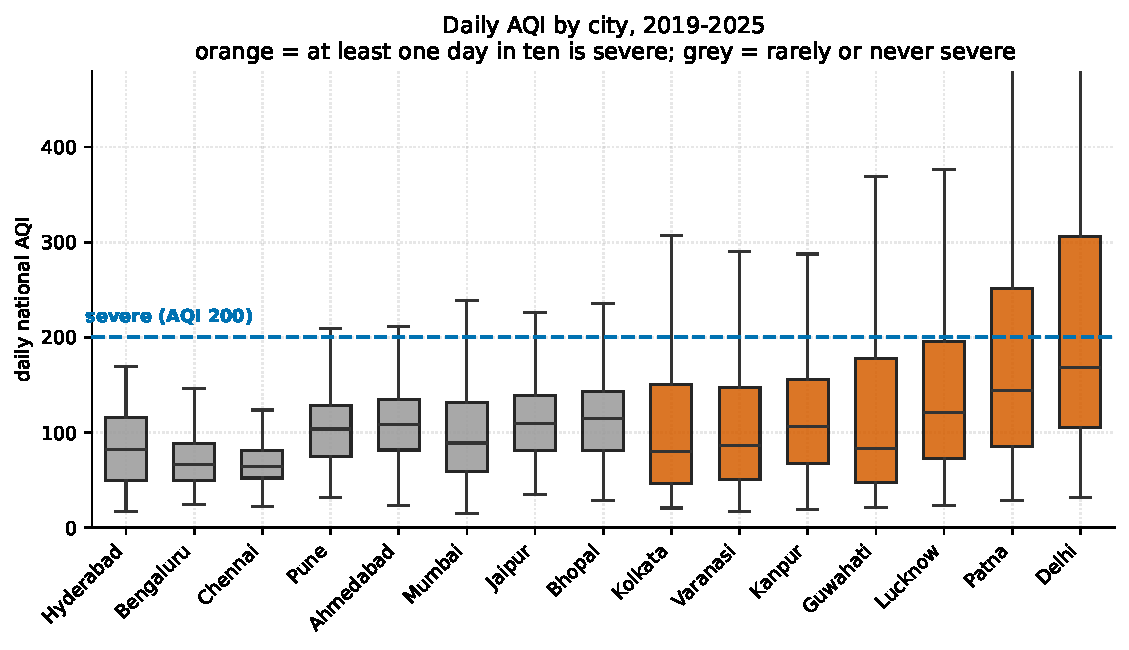
\includegraphics[width=0.92\textwidth]{figA_city_aqi.pdf}
\caption{Daily AQI by city, 2019--2025, against the severe line at AQI 200. Orange marks
cities severe on at least one day in ten. The grey cities cannot support a severe-day
ranking metric, which is why they are absent from Table~\ref{tab:percity}.}
\label{fig:cityaqi}
\end{figure*}

\begin{figure}[t]
\centering
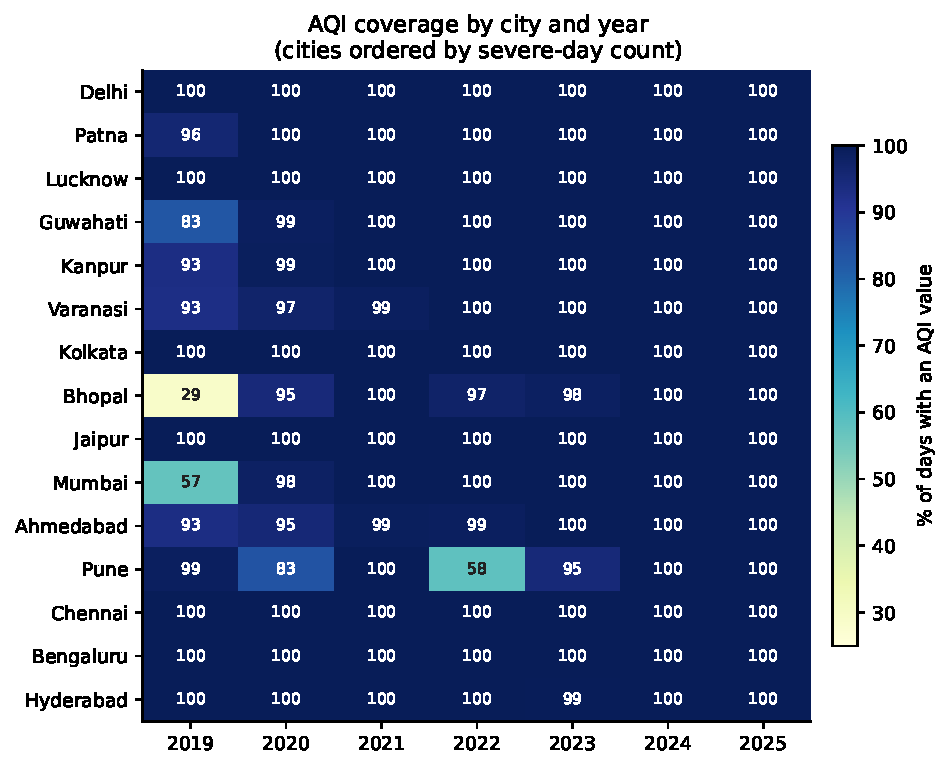
\includegraphics[width=\columnwidth]{figB_coverage.pdf}
\caption{Share of days with an AQI value, by city and year. Coverage is essentially
complete from 2021 onwards.}
\label{fig:coverage}
\end{figure}

\subsection{Leave-one-city-out protocol}

Table~\ref{tab:loco} states the protocol. In each of fifteen folds, the other fourteen
cities train on 2019--2023 (25{,}564 city-days) and validate on 2024 (5{,}124 city-days);
the held-out city alone is scored on 2024--2025 (731 days). The held-out city contributes
nothing to training, to validation, to the gap-filling medians or to the alarm
thresholds; its own history reaches a forecast only as the input a forecaster would
genuinely possess on the day. Because training ends on 2023-12-31 and evaluation begins
on 2024-01-01, the holdout is simultaneously spatial and temporal.

\begin{table*}[t]
\centering
\caption{The leave-one-city-out protocol. In each of the fifteen folds the other fourteen cities train on 2019--2023 and validate on 2024, and the held-out city alone is scored on 2024--2025; it contributes nothing to training, validation, gap-filling medians or alarm levels. Severe days are days above AQI 200 in the held-out period. The per-city results table instead counts severe forecast \emph{targets} in the complete-case evaluation frame, where each day appears once per horizon, so its counts differ by construction.}
\label{tab:loco}

\footnotesize
\resizebox{\ifdim\width>\textwidth\textwidth\else\width\fi}{!}{%
\begin{tabular}{lrrrrr}
\toprule
held-out city & train days & val days & test days & test severe & test severe (\%) \\
\midrule
Delhi & 25564 & 5124 & 731 & 272 & 37.2 \\
Patna & 25564 & 5124 & 731 & 184 & 25.2 \\
Guwahati & 25564 & 5124 & 731 & 123 & 16.8 \\
Lucknow & 25564 & 5124 & 731 & 82 & 11.2 \\
Bhopal & 25564 & 5124 & 731 & 70 & 9.6 \\
Jaipur & 25564 & 5124 & 731 & 55 & 7.5 \\
Kolkata & 25564 & 5124 & 731 & 55 & 7.5 \\
Pune & 25564 & 5124 & 731 & 42 & 5.7 \\
Kanpur & 25564 & 5124 & 731 & 17 & 2.3 \\
Mumbai & 25564 & 5124 & 731 & 16 & 2.2 \\
Ahmedabad & 25564 & 5124 & 731 & 6 & 0.8 \\
Chennai & 25564 & 5124 & 731 & 4 & 0.5 \\
Varanasi & 25564 & 5124 & 731 & 2 & 0.3 \\
Hyderabad & 25564 & 5124 & 731 & 0 & 0.0 \\
Bengaluru & 25564 & 5124 & 731 & 0 & 0.0 \\
\bottomrule
\end{tabular}%
}
\end{table*}


Forecasts are produced at horizons of one, two and three days. Every learned model uses
early stopping on the validation split, and all scaling statistics and imputation
medians are computed on training rows only.

% =====================================================================
\section{Method}
\label{sec:method}
% =====================================================================

\subsection{Anchoring}

A forecaster for a city it has never seen cannot rely on learned local climatology. The
single most informative quantity available is the city's own most recent observation.
We therefore predict a \emph{correction} to an anchor rather than an absolute level:
the output head is zero-initialised so that the model begins life as a persistence
forecast and must earn every departure from it.

We evaluate a ladder of anchor variants, one change per rung, reported in
Fig.~\ref{fig:ladder}: anchors supplied only as inputs; an anchor token with a
mean start (RevIN-style); a learned mixture of the fortnight mean and today; and the
full anchored forecast.

\subsection{The nightly anchor}

\todo{define precisely: which hours, how the previous night's concentrations are
aggregated, and why the night before is informative for the following day.} The nightly
anchor requires no training and no severe day from the city, which makes it the natural
reference for a city with no monitoring record.

\subsection{Sub-daily tokens}

The daily AQI is a summary of a shape. Two cities with identical daily means can differ
sharply in how concentration accumulates overnight and ventilates after sunrise. We
supply the model with 72 hours of sub-daily pollutant channels as additional tokens.

\subsection{Model selection}

Selection was performed on validation rows only, before any held-out value was read.
Table~\ref{tab:selection} shows the five candidates; the selected model attained both the
lowest validation RMSE and the highest validation average precision, so no tie-break was
required.

\begin{table}[t]
\centering
\caption{Candidate selection on validation rows only. The pre-registered rule picks the lowest validation RMSE among candidates within 0.002 average precision of the control.}
\label{tab:selection}
\begin{tabular}{lrr}
\toprule
model & validation RMSE & validation AP \\
\midrule
control & 32.167 & 0.732 \\
anchor\_inputs & 32.108 & 0.732 \\
anchored & 32.014 & 0.734 \\
multires & 31.906 & 0.736 \\
\textbf{dextra} & \textbf{31.737} & \textbf{0.738} \\
\bottomrule
\end{tabular}
\end{table}


% =====================================================================
\section{Results}
\label{sec:results}
% =====================================================================

\subsection{Reporting against an error floor}

Raw RMSE is hard to interpret because an unknown part of the error is irreducible:
measurement noise and genuine unpredictability. We estimate that floor from repeated
measurement of the same city-days and obtain 15.44 AQI RMSE at the next-day horizon. We
then report, for each forecaster, the share of the \emph{removable} error it removes,
\begin{equation}
\text{share} = \frac{\mathrm{RMSE}_{\text{persist}}^{2} - \mathrm{RMSE}_{f}^{2}}
                    {\mathrm{RMSE}_{\text{persist}}^{2} - \mathrm{RMSE}_{\text{floor}}^{2}},
\label{eq:share}
\end{equation}
so that persistence sits at 0 and the floor at 1. Fig.~\ref{fig:ceiling} and
Table~\ref{tab:noise} give the result.

\begin{figure*}[t]
\centering
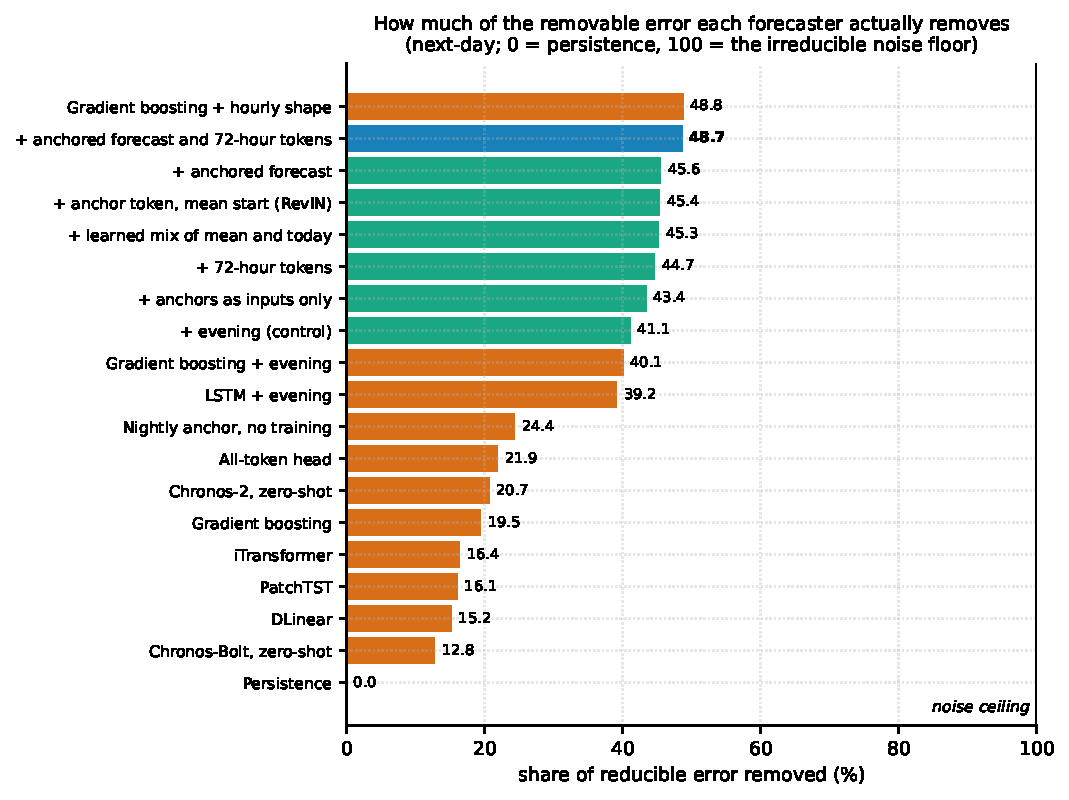
\includegraphics[width=0.86\textwidth]{fig1_noise_ceiling.pdf}
\caption{Share of removable next-day error each forecaster removes, by
(\ref{eq:share}). Persistence is 0 and the estimated noise floor is 100. Gradient
boosting with the same sub-daily features (48.8\%) is indistinguishable from the proposed
model (48.7\%).}
\label{fig:ceiling}
\end{figure*}

\begin{table*}[t]
\centering
\caption{Next-day error against the estimated irreducible noise floor.}
\label{tab:noise}
\footnotesize
\resizebox{\ifdim\width>\textwidth\textwidth\else\width\fi}{!}{%
\begin{tabular}{lrrrrr}
\toprule
forecaster & next-day RMSE & next-day AP & next-day onset AP & share of squared error that is noise & share of reducible error removed \\
\midrule
noise ceiling (no forecaster can pass this) & 15.439 & 0.952 & 0.835 & 1.000 & 1.000 \\
Persistence & 29.140 & 0.775 & 0.245 & 0.281 & 0.000 \\
Nightly anchor, no training & 26.463 & 0.810 & 0.314 & 0.340 & 0.244 \\
Gradient boosting & 27.023 & 0.788 & 0.293 & 0.326 & 0.195 \\
Gradient boosting + evening & 24.582 & 0.822 & 0.364 & 0.394 & 0.401 \\
Gradient boosting + hourly shape & 23.479 & 0.846 & 0.413 & 0.432 & 0.488 \\
DLinear & 27.499 & 0.796 & 0.288 & 0.315 & 0.152 \\
PatchTST & 27.403 & 0.797 & 0.280 & 0.317 & 0.161 \\
LSTM + evening & 24.696 & 0.831 & 0.404 & 0.391 & 0.392 \\
Chronos-Bolt, zero-shot & 27.768 & 0.795 & 0.294 & 0.309 & 0.128 \\
Chronos-2, zero-shot & 26.889 & 0.807 & 0.306 & 0.330 & 0.207 \\
iTransformer & 27.368 & 0.795 & 0.272 & 0.318 & 0.164 \\
All-token head & 26.742 & 0.811 & 0.346 & 0.333 & 0.219 \\
+ evening (control) & 24.451 & 0.837 & 0.379 & 0.399 & 0.411 \\
+ anchors as inputs only & 24.164 & 0.835 & 0.359 & 0.408 & 0.434 \\
+ anchor token, mean start (RevIN) & 23.912 & 0.843 & 0.380 & 0.417 & 0.454 \\
+ learned mix of mean and today & 23.931 & 0.840 & 0.378 & 0.416 & 0.453 \\
+ anchored forecast & 23.894 & 0.842 & 0.379 & 0.417 & 0.456 \\
+ 72-hour tokens & 24.007 & 0.843 & 0.405 & 0.414 & 0.447 \\
\textbf{+ anchored forecast and 72-hour tokens} & \textbf{23.492} & \textbf{0.844} & \textbf{0.392} & \textbf{0.432} & \textbf{0.487} \\
\bottomrule
\end{tabular}%
}
\end{table*}


Persistence attains 29.14 AQI RMSE at one day and the proposed model 23.49, which is
48.7\% of the removable error. The training-free nightly anchor alone reaches 24.4\%,
and both zero-shot foundation models fall below it (Chronos-2, 20.7\%; Chronos-Bolt,
12.8\%), as do DLinear (15.2\%), PatchTST (16.1\%) and the inverted transformer (16.4\%)
when given daily inputs only.

\subsection{Severe-day ranking}

Because severe days are rare and an alarm threshold is an arbitrary choice --- one whose
selection alone moved a single city's F1 from 0.41 to 0.09 in preliminary work --- we
score severe-day detection with average precision (AP), which is threshold-free.
Table~\ref{tab:scores} reports pooled results and Table~\ref{tab:verdict} the paired
comparisons.

\begin{table*}[t]
\centering
\caption{Leave-one-city-out results across all fifteen cities, three seeds.}
\label{tab:scores}
\footnotesize
\resizebox{\ifdim\width>\textwidth\textwidth\else\width\fi}{!}{%
\begin{tabular}{lrrrrrr}
\toprule
forecaster & AP & onset AP & next-day AP & RMSE & next-day RMSE & onsets caught \\
\midrule
Persistence & 0.684 & 0.197 & 0.775 & 36.644 & 29.140 & 31.000 \\
Nightly anchor, no training & 0.700 & 0.216 & 0.810 & 35.663 & 26.463 & 41.000 \\
Gradient boosting & 0.709 & 0.306 & 0.788 & 33.283 & 27.023 & 98.000 \\
Gradient boosting + evening & 0.726 & 0.320 & 0.822 & 32.042 & 24.582 & 103.000 \\
Gradient boosting + hourly shape & 0.741 & 0.327 & 0.846 & 31.608 & 23.479 & 103.000 \\
DLinear & 0.731 & 0.276 & 0.796 & 32.915 & 27.499 & 67.667 \\
PatchTST & 0.733 & 0.273 & 0.797 & 32.810 & 27.403 & 51.333 \\
LSTM + evening & 0.760 & 0.350 & 0.831 & 30.988 & 24.696 & 93.333 \\
Chronos-Bolt, zero-shot & 0.727 & 0.270 & 0.795 & 33.325 & 27.768 & 76.000 \\
Chronos-2, zero-shot & 0.752 & 0.310 & 0.807 & 31.599 & 26.889 & 81.000 \\
iTransformer & 0.730 & 0.266 & 0.795 & 32.758 & 27.368 & 78.000 \\
All-token head & 0.753 & 0.325 & 0.811 & 31.916 & 26.742 & 84.667 \\
+ evening (control) & 0.760 & 0.331 & 0.837 & 31.045 & 24.451 & 94.333 \\
+ anchors as inputs only & 0.759 & 0.325 & 0.835 & 30.922 & 24.164 & 101.667 \\
+ anchor token, mean start (RevIN) & 0.764 & 0.333 & 0.843 & 30.801 & 23.912 & 94.667 \\
+ learned mix of mean and today & 0.763 & 0.333 & 0.840 & 30.796 & 23.931 & 104.333 \\
+ anchored forecast & 0.763 & 0.330 & 0.842 & 30.872 & 23.893 & 96.000 \\
+ 72-hour tokens & 0.762 & 0.345 & 0.843 & 30.838 & 24.006 & 106.000 \\
\textbf{+ anchored forecast and 72-hour tokens} & \textbf{0.763} & \textbf{0.343} & \textbf{0.844} & \textbf{30.672} & \textbf{23.492} & \textbf{108.667} \\
\bottomrule
\end{tabular}%
}
\end{table*}

\begin{table*}[t]
\centering
\caption{The final model against each rival, with Holm-corrected p-values. Intervals spanning zero are reported as ties.}
\label{tab:verdict}
\footnotesize
\resizebox{\ifdim\width>\textwidth\textwidth\else\width\fi}{!}{%
\begin{tabular}{lrrrrr}
\toprule
final against & AP difference & AP 95\% & AP p (Holm) & RMSE difference & RMSE p (Holm) \\
\midrule
Persistence & 0.079 & [+0.056, +0.122] & 0.036 & -5.971 & 0.036 \\
Nightly anchor, no training & 0.064 & [+0.042, +0.116] & 0.036 & -4.990 & 0.036 \\
Gradient boosting & 0.054 & [+0.023, +0.154] & 0.048 & -2.610 & 0.036 \\
Gradient boosting + evening & 0.037 & [-0.012, +0.104] & 0.783 & -1.370 & 0.040 \\
Gradient boosting + hourly shape & 0.022 & [-0.019, +0.079] & 1.000 & -0.936 & 0.084 \\
DLinear & 0.032 & [+0.026, +0.054] & 0.036 & -2.242 & 0.036 \\
PatchTST & 0.030 & [+0.023, +0.052] & 0.036 & -2.137 & 0.036 \\
LSTM + evening & 0.004 & [-0.002, +0.020] & 0.687 & -0.316 & 0.036 \\
Chronos-Bolt, zero-shot & 0.036 & [+0.023, +0.049] & 0.036 & -2.652 & 0.036 \\
Chronos-2, zero-shot & 0.011 & [+0.002, +0.031] & 0.306 & -0.927 & 0.036 \\
iTransformer & 0.033 & [+0.025, +0.058] & 0.036 & -2.086 & 0.036 \\
All-token head & 0.011 & [+0.004, +0.052] & 0.066 & -1.243 & 0.036 \\
+ evening (control) & 0.003 & [-0.005, +0.017] & 0.815 & -0.372 & 0.036 \\
+ anchors as inputs only & 0.004 & [+0.001, +0.021] & 0.220 & -0.249 & 0.036 \\
+ anchor token, mean start (RevIN) & -0.001 & [-0.005, +0.014] & 1.000 & -0.128 & 0.084 \\
+ learned mix of mean and today & -0.000 & [-0.004, +0.014] & 1.000 & -0.124 & 0.084 \\
+ anchored forecast & 0.000 & [-0.003, +0.019] & 1.000 & -0.200 & 0.036 \\
+ 72-hour tokens & 0.001 & [-0.002, +0.007] & 1.000 & -0.166 & 0.040 \\
\bottomrule
\end{tabular}%
}
\end{table*}


The pre-registered primary outcome is the proposed model against persistence on
severe-day AP. It passes: $\Delta\mathrm{AP} = +0.0788$, 95\% CI $[+0.056, +0.122]$,
Holm-corrected $p = 0.036$. Onset detection, the harder task of catching the first day of
an episode, improves from AP 0.197 to 0.343, and the number of episode onsets caught rises
from 31 to 109.

\subsection{A note on the $p$-values}
\label{sec:pvalues}

Several comparisons in Table~\ref{tab:verdict} report $p = 0.036$ exactly. Intervals and
$p$-values come from resampling whole held-out cities with $B = 1000$ draws, and the
two-sided $p$ is computed as $2(k+1)/(B+1)$ where $k$ is the number of draws on the
opposite side of zero. The smallest attainable raw value is therefore
$2/1001 = 0.002$, which after Holm correction across the 18 comparisons becomes 0.036.
A comparison reported at 0.036 is thus one whose sign \emph{never reversed in any
resample}, not a marginal one. Note also that the confidence intervals are
per-comparison while the $p$-values are Holm-corrected across the family, which is why a
few rows show an interval excluding zero alongside $p > 0.05$.

\subsection{The architecture does not carry the gain}

Fig.~\ref{fig:verdict} summarises what the proposed model beats and what it merely ties.
It is significantly better than persistence, the nightly anchor, plain gradient boosting,
the inverted transformer, DLinear, PatchTST and Chronos-Bolt. It \emph{ties} with gradient
boosting given evening features, gradient boosting given the hourly shape, the LSTM given
evening features, Chronos-2 and the all-token head.

\begin{figure*}[t]
\centering
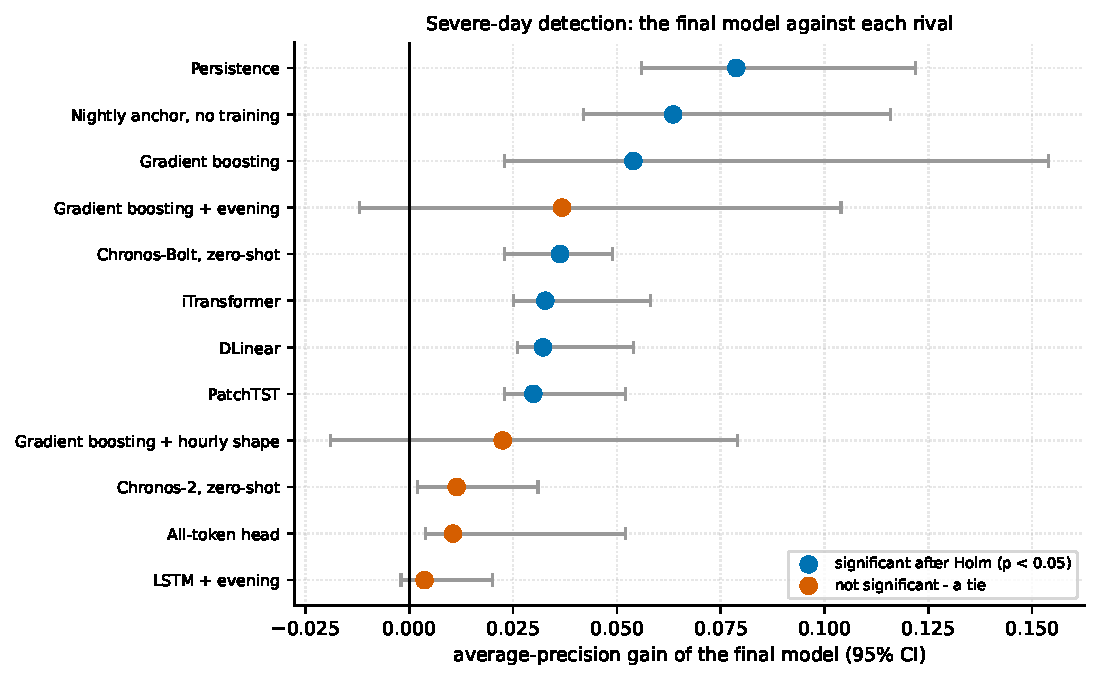
\includegraphics[width=0.86\textwidth]{fig2_verdict_forest.pdf}
\caption{Paired differences in severe-day average precision against each rival, with 95\%
intervals from resampling whole held-out cities. Intervals crossing zero are ties.}
\label{fig:verdict}
\end{figure*}

The tie that matters is with gradient boosting given the hourly shape: 48.8\% against
48.7\% on (\ref{eq:share}), and $\Delta\mathrm{AP} = +0.022$ with a 95\% interval of
$[-0.019, +0.079]$ that comfortably spans zero. Per city the split is even: the proposed
model is ahead in Delhi, Guwahati, Lucknow and Pune, and behind in Patna, Bhopal, Jaipur
and Kolkata (Table~\ref{tab:percity}).

We therefore do not claim an architectural advance. The defensible claim is about
\emph{information}: supplying any competent learner with sub-daily pollutant shape, and
anchoring its forecast on the most recent observation, is what moves the result.
Fig.~\ref{fig:ladder} shows the ablation ladder, in which each rung changes exactly one
thing.

\begin{figure*}[t]
\centering
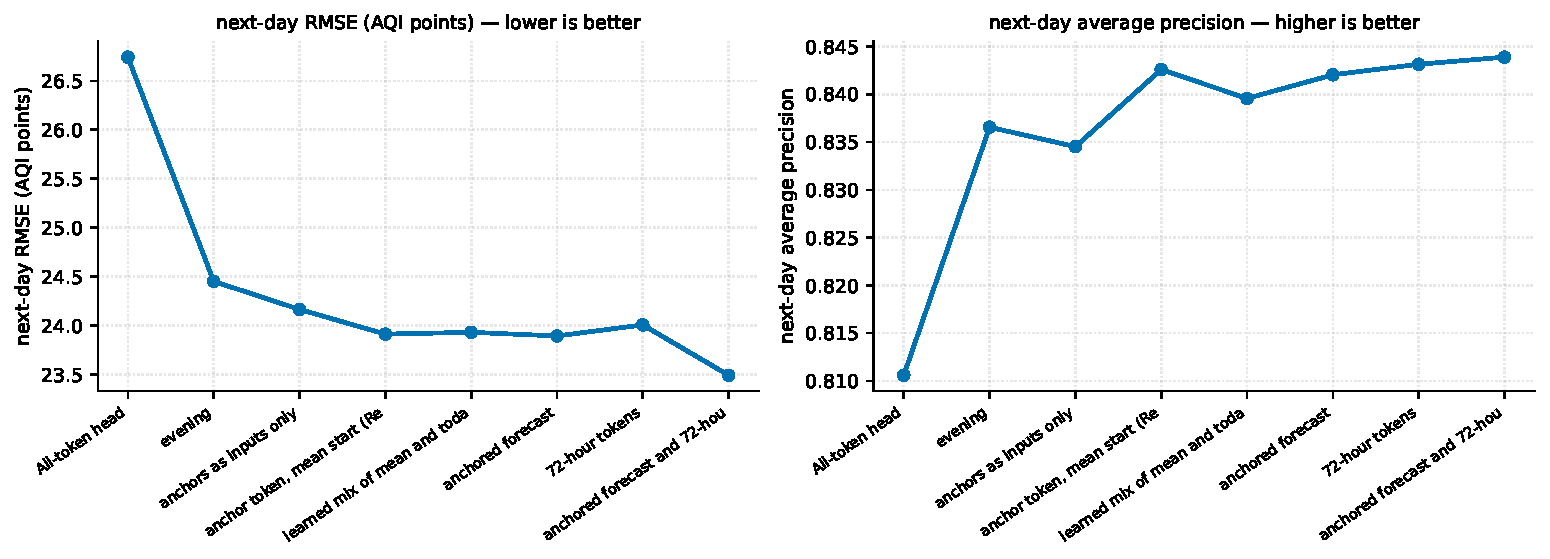
\includegraphics[width=0.86\textwidth]{fig3_ablation_ladder.pdf}
\caption{The ablation ladder: one change per rung, from the evening-feature control to
the full anchored forecast with 72-hour tokens.}
\label{fig:ladder}
\end{figure*}

% =====================================================================
\section{Per-City Behaviour and Limitations}
\label{sec:percity}
% =====================================================================

\begin{table*}[t]
\centering
\caption{Severe-day average precision for each held-out city.}
\label{tab:percity}
\footnotesize
\resizebox{\ifdim\width>\textwidth\textwidth\else\width\fi}{!}{%
\begin{tabular}{lrrrrrrrr}
\toprule
city & severe & onsets & AP persistence & AP nightly anchor & AP gbm hourly & AP chronos-2 & AP control & AP final \\
\midrule
Delhi & 591.000 & 87.000 & 0.896 & 0.906 & 0.934 & 0.930 & 0.937 & 0.939 \\
Patna & 183.000 & 107.000 & 0.461 & 0.475 & 0.591 & 0.531 & 0.545 & 0.561 \\
Guwahati & 123.000 & 62.000 & 0.499 & 0.504 & 0.533 & 0.532 & 0.541 & 0.541 \\
Bhopal & 66.000 & 45.000 & 0.259 & 0.277 & 0.372 & 0.322 & 0.313 & 0.339 \\
Lucknow & 48.000 & 41.000 & 0.160 & 0.197 & 0.270 & 0.244 & 0.271 & 0.281 \\
Pune & 41.000 & 20.000 & 0.567 & 0.571 & 0.605 & 0.585 & 0.638 & 0.637 \\
Jaipur & 27.000 & 23.000 & 0.075 & 0.094 & 0.099 & 0.068 & 0.075 & 0.097 \\
Kolkata & 12.000 & 11.000 & 0.071 & 0.083 & 0.116 & 0.171 & 0.092 & 0.108 \\
\bottomrule
\end{tabular}%
}
\end{table*}


\begin{figure}[t]
\centering
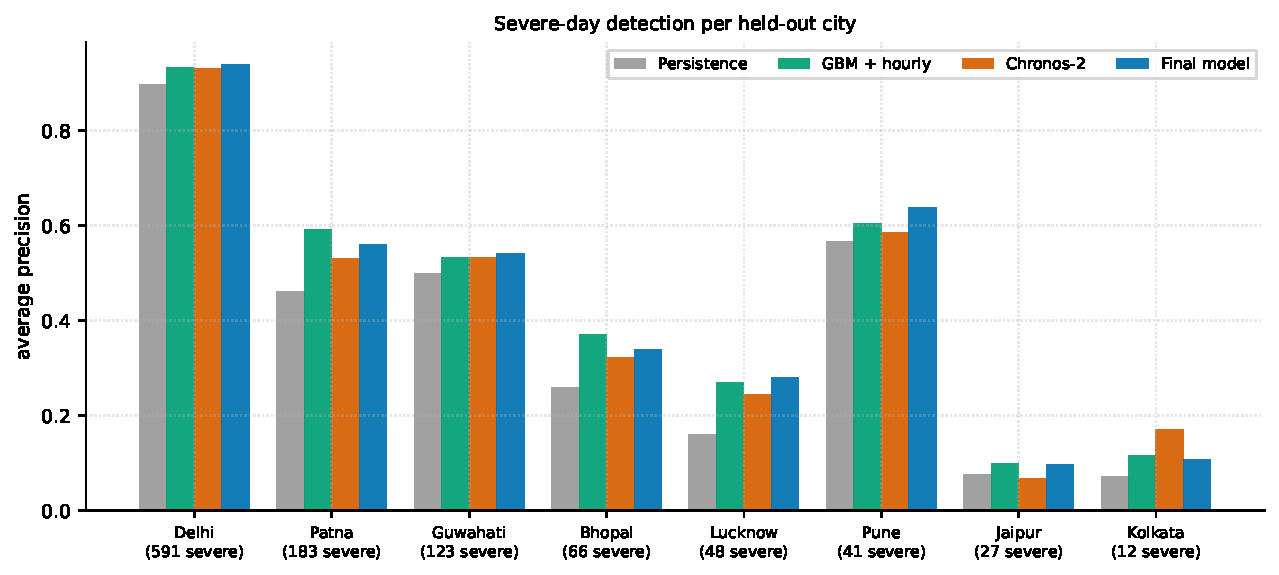
\includegraphics[width=\columnwidth]{fig4_per_city.pdf}
\caption{Severe-day average precision per held-out city, with severe-day counts. Cities
with too few severe targets to estimate AP are omitted.}
\label{fig:percity}
\end{figure}

\textbf{Not every city can be scored.} Average precision is undefined without positives.
As Table~\ref{tab:loco} shows, the held-out period contains 272 severe days for Delhi but
only two for Varanasi and \emph{none at all} for Hyderabad or Bengaluru. We therefore
report per-city AP only for cities with at least ten severe targets in the evaluation
frame. Note that Table~\ref{tab:loco} counts severe \emph{days} whereas
Table~\ref{tab:percity} counts severe \emph{targets} in the complete-case evaluation
frame, in which each day appears once per horizon and rows lacking any forecaster are
dropped; for Delhi these are 272 and 591 respectively.

\textbf{Delhi dominates the pooled numbers, but the conclusion survives its removal.}
Pooled severe-day AP falls from 0.763 to 0.441 when Delhi is excluded, simply because the
remaining cities have far lower severe base rates. The \emph{margin} over persistence,
however, widens rather than narrows: $+0.079$ pooled against $+0.102$ without Delhi. The
finding is therefore not an artefact of one city.

\textbf{The archive is a subset of the network.} At most six reporting stations per city
appear in the assembled record, against nominal CAAQMS networks several times larger for
the biggest cities. City-level AQI is correspondingly a sparser average than the full
network would give. \todo{confirm whether the CPCB download covered all stations, and
state the conclusion here either way.}

\textbf{Scope.} \todo{state that the pre-registered 2026 confirmatory test is planned and
has not been run, and that the results reported here are the leave-one-city-out results on
2024--2025.}

% =====================================================================
\section{Operational Value}
% =====================================================================

A ranking metric is not an operational one. Fig.~\ref{fig:onsets} reports episode onsets
caught --- the first day of a severe run, which is the day an advisory would have to be
issued to be useful. The proposed model catches 109 of them against persistence's 31,
with alarm thresholds tuned on validation cities only.

\begin{figure}[t]
\centering
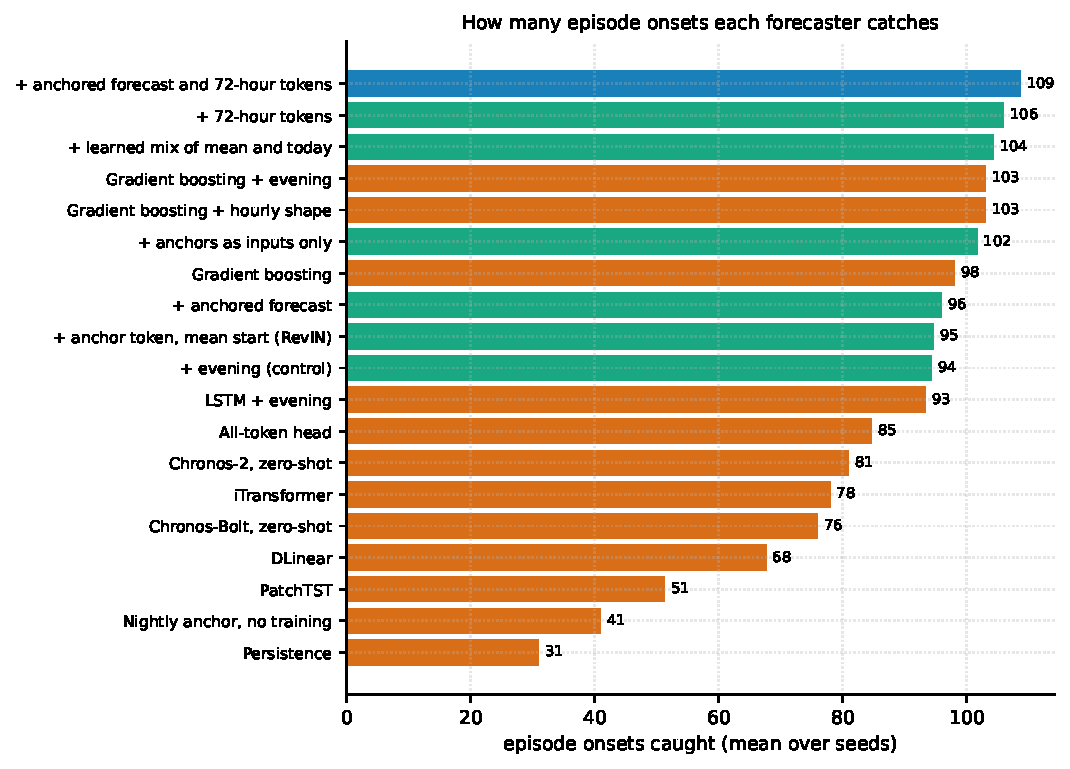
\includegraphics[width=\columnwidth]{fig5_onsets.pdf}
\caption{Episode onsets caught. An onset is the first day of a severe run, the day on
which an advisory must be issued to have value.}
\label{fig:onsets}
\end{figure}

\todo{one paragraph translating this into practice: what lead time an advisory needs, and
what a false-alarm rate of this magnitude costs.}

% =====================================================================
\section{Conclusion}
% =====================================================================

Evaluated on cities it has never seen, a forecaster anchored on the most recent
observation and supplied with 72 hours of sub-daily pollutant shape removes 48.7\% of the
removable next-day error and raises severe-day average precision by 0.079 over
persistence. The same features given to gradient boosting perform identically, so we
attribute the gain to the information rather than to the architecture. For a city with no
monitoring history at all, a training-free nightly anchor already recovers roughly a
quarter of the removable error, which we suggest is the appropriate baseline for future
work on transfer in this setting.

\todo{one sentence on future work: the planned 2026 confirmatory test, and folding the
CPCB sub-index rule into the network output layer.}

\section*{Acknowledgements}

Pollutant data derive from the Central Pollution Control Board (CPCB) CAAQMS network.
Meteorological data are from ERA5 / Copernicus Climate Change Service (CC-BY) and
Open-Meteo (CC-BY 4.0). Fire activity is from NASA FIRMS.
\todo{add CPCB permission statement once approval is received.}

% =====================================================================
% VERIFY EVERY ENTRY BELOW BEFORE SUBMITTING, AND ADD THE DOMAIN LITERATURE.
% =====================================================================
\begin{thebibliography}{00}

\bibitem{nie2023patchtst} Y. Nie, N. H. Nguyen, P. Sinthong, and J. Kalagnanam,
``A time series is worth 64 words: Long-term forecasting with transformers,''
in \emph{Proc. Int. Conf. Learn. Represent. (ICLR)}, 2023.

\bibitem{liu2024itransformer} Y. Liu, T. Hu, H. Zhang, H. Wu, S. Wang, L. Ma, and
M. Long, ``iTransformer: Inverted transformers are effective for time series
forecasting,'' in \emph{Proc. Int. Conf. Learn. Represent. (ICLR)}, 2024.

\bibitem{zeng2023dlinear} A. Zeng, M. Chen, L. Zhang, and Q. Xu,
``Are transformers effective for time series forecasting?,''
in \emph{Proc. AAAI Conf. Artif. Intell.}, 2023.

\bibitem{ansari2024chronos} A. F. Ansari \emph{et al.},
``Chronos: Learning the language of time series,''
\emph{Trans. Mach. Learn. Res. (TMLR)}, 2024.

\bibitem{ke2017lightgbm} G. Ke \emph{et al.},
``LightGBM: A highly efficient gradient boosting decision tree,''
in \emph{Adv. Neural Inf. Process. Syst. (NeurIPS)}, 2017.

\bibitem{cpcb2014naqi} Central Pollution Control Board,
``National Air Quality Index,'' Government of India, Tech. Rep., 2014.

\end{thebibliography}

\end{document}
